% !TEX root = ReviewDraft.tex


\section{Preliminaries}

\subsection{Black hole thermodynamics}
When an object is dropped into a black hole, the black hole responds dynamically. The event horizon ripples briefly, and then quickly settles down to a new equilibrium at a larger radius. It was noticed in the 1970s that the resulting small changes in the black hole geometry are constrained by equations  closely parallel to the laws of thermodynamics \cite{Christodoulou:1970wf,Christodoulou:1972kt,Hawking:1971tu,Bekenstein:1972tm,Bekenstein:1973ur,carter1972rigidity,Bardeen:1973gs,Hawking:1974rv,Hawking:1974sw}. The equation governing the response of a rotating black hole is \cite{Bardeen:1973gs}
\be
\frac{\kappa}{8\pi \GN} d\left( \mbox{Area} \right)  = dM  - \Omega dJ \ ,
\ee
where $\kappa$ is its surface gravity\footnote{Unfortunately, the name ``surface gravity'' is a bit misleading since the proper acceleration of an observer hovering at the horizon is infinite. $\kappa$ is related to the force on a massless (unphysical) string at infinity, see e.g. \cite{Wald:1984rg}.}, $M$ is its mass, $J$ is its angular momentum, and $\Omega$ is the rotational velocity of the horizon. The area refers to the area of the event horizon, and $\GN$ is Newton's constant.
If we postulate that the black hole has temperature $T \propto \kappa$, and entropy $S_{\rm BH} \propto \mbox{Area}$, then this looks identical to the first law of thermodynamics in the form
\be\label{firstlaw}
TdS_{\rm BH} = dM - \Omega dJ \ .
\ee
In addition, the area of the horizon always increases in the classical theory \cite{Hawking:1971tu}, suggesting a connection to the second law of thermodynamics. 
This is just a rewriting of the Einstein equations in suggestive notation, and initially, there was little reason to believe that it had anything to do with `real' thermodynamics. In classical general relativity, black holes have neither a temperature nor any significant entropy.  This changed with Hawking's discovery that,  when general relativity is coupled to quantum field theory, black holes have a temperature \cite{Hawking:1974sw}
\be
T = \frac{\hbar \kappa}{2\pi } \ .
\ee
(We set $c=k_B = 1$.) This formula for the temperature fixes the proportionality constant in $S_{\rm BH} \propto \mbox{Area}$. The total entropy of a black hole and its environment also has a contribution from the quantum fields outside the horizon. This suggests that the total or `generalized' entropy of a black hole is \cite{Bekenstein:1973ur}
\be\label{sgen}
S_{\rm gen} = \frac{\mbox{Area of horizon}}{4 \hbar \GN} + S_{\rm outside}  \ , \ee
where $S_{\rm outside}$ denotes the entropy of  matter  as well as gravitons outside the black hole, as it appears in the semiclassical description. It also includes a vacuum contribution from the quantum fields \cite{Bombelli:1986rw}.\footnote{  The quantum  contribution by itself has an ultraviolet divergence from the short distance entanglement of quantum fields across the horizon. This piece is proportional to the area, $A/\epsilon_{uv}^2$.  However, matter loops also lead to an infinite renormalization of Newton's constant, $1/(4 G_N) \to { 1 \over 4 G_N} - { 1 \over \epsilon^2_{uv}}$.  Then these two effects cancel each other so that $S_{\rm gen}$ is finite.   As usual in effective theories, these formally ``infinite'' quantities are actually subleading when we remember that we should take a small cutoff but not too small, $l_p \ll \epsilon_{uv} \ll r_s$. } 
The generalized entropy, including this quantum term, is also found to obey the second law of thermodynamics \cite{Wall:2011hj}, 
\be
\Delta S_{\rm gen} \geq 0 \ ,
\ee
giving further evidence that it is really an entropy. This result is stronger than the classical area theorem because it also covers phenomena like Hawking radiation, when the area decreases but the generalized entropy increases due to the entropy of Hawking radiation. 

The area is measured in Planck units, $l_p^2 = \hbar \GN$, so if this entropy has an origin in statistical mechanics then a black hole must have an enormous number of degrees of freedom. For example, the black hole at the center of the Milky Way,   Sagittarius A*,  has
\be
S  \approx {10^{85}} \ .  
\ee
Even for a black hole the size of a proton, $S \approx 10^{40}$.
In classical general relativity, according to the no-hair theorem, there is just one black hole with mass $M$ and angular momentum $J$, so the statistical entropy of a black hole is naively zero. 
 Including quantum fields helps, but has not led to a successful accounting of the entropy. 
 Finding explicitly the states giving rise to the entropy is an interesting problem, which we will not discuss in this review. 


\subsection{Hawking radiation}


The metric of a Schwarzschild black hole is
\be\label{schw}
ds^2 = -\left( 1 - \frac{r_s}{r} \right) dt^2 + \frac{dr^2}{1 - \frac{r_s}{r}} + r^2 d\Omega_2^2 \ .
\ee
The Schwarzschild radius  $r_s = 2\GN M$ sets the size of the black hole. We will ignore the angular directions $d\Omega_2^2$ which do not play much of a role. To zoom in on the event horizon, we change coordinates, $r \to r_s(1 + \frac{\rho^2}{4r_s^2})$, $t \to 2 r_s \tau$, and expand for $\rho \ll r_s$. This gives the near-horizon metric
\be \la{RescMe}
ds^2 \approx  -\rho^2 d\tau^2 + d\rho^2 \ .
\ee
To this approximation, this is just flat Minkowski spacetime. To see this, define the new coordinates
\be\label{rindlerc}
x^0 = \rho \sinh \tau , \qquad x^1 = \rho \cosh \tau
\ee
in which 
\be \la{LocMin}
ds^2\approx  -\rho^2 d\tau^2 + d\rho^2  = -(dx^0)^2 + (dx^1)^2 \ .
\ee
Therefore according to a free-falling observer, the event horizon $r=r_s$ is not special. It is just like any other point in a smooth spacetime, and in particular, the geometry extends smoothly past the horizon into the black hole. This is a manifestation of the equivalence principle: free-falling observers do not feel the effect of gravity.  Of course, an observer that crosses the horizon will not be able to send signals to the outside\footnote{We can say that the interior lies behind a Black Shield (or Schwarz Schild in German).}.


The spacetime geometry of a Schwarzschild black hole that forms by gravitational collapse is illustrated in fig.~\ref{fig:schwarzschild}. An observer hovering near the event horizon at fixed $r$ is accelerating --- a rocket is required to avoid falling in. In the near-horizon coordinates \nref{LocMin}, an observer at fixed $\rho$ is following  the trajectory of a uniformly accelerated observer in Minkowski spacetime.


\begin{figure}[t]
\begin{center}
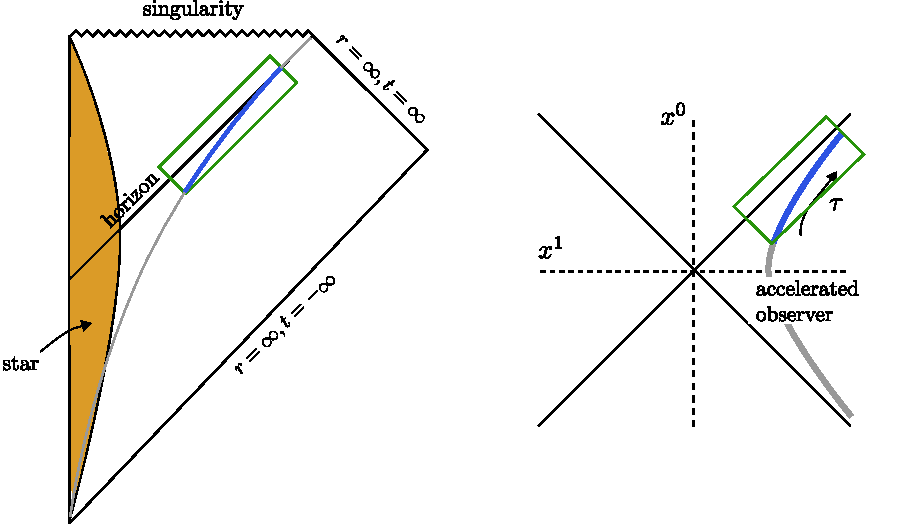
\includegraphics[scale=1]{figures/collapse-penrose.pdf}
\end{center}
\caption{\small Left: Penrose diagram of a black hole formed by gravitational collapse.  Right: Zoomed-in view of the flat near-horizon region, with the trajectory of a uniformly accelerated observer at $\rho = a^{-1}$.
\label{fig:schwarzschild}}
\end{figure}



A surprising fact is that a uniformly accelerating observer in flat space detects thermal radiation. 
This is known as the Unruh effect \cite{Unruh:1976db}. There is a simple trick to obtain the temperature \cite{Bisognano:1976za}. The coordinate change \eqref{rindlerc} is very similar to the usual coordinate change from Cartesian coordinates to polar coordinates. It becomes identical if we perform the Wick rotation $\tau = i \theta$, $x^0 = i x^0_E$; then
\be
x^0_E = \rho \sin \theta , \quad x^1 = \rho \cos\theta \ .
\ee
The new coordinates $(x^0_E, x^1)$ or $(\rho, \theta)$ are simply Cartesian or polar coordinates on the Euclidean plane $\mathbb{R}^2$. 
In Euclidean space, an observer at constant $\rho$ moves in a circle of length $ 2\pi \rho$. 
Euclidean time evolution on a circle is related to the computation of thermodynamic quantities for the original physical system (we will return to this in section \ref{ss:gibbonshawking}). 
Namely, $\tr[e^{ - \beta H}] $ is the partition function at temperature $T=1/\beta$. $\beta$ is the length of the Euclidean time evolution and the trace is related to the fact that we are on a circle. This suggests that the temperature that an accelerated observer feels is 
\be \la{PropT}
T_{proper} = { 1 \over 2 \pi \rho } = { a \over 2 \pi } = { \hbar \over k_B c } { a \over 2 \pi } 
\ee 
where $a$ is the proper acceleration and we also restored all the units in the last formula. 
Though this argument seems a bit formal, one can check that a physical accelerating thermometer would actually record this temperature \cite{Unruh:1976db}. 

Now, this is the proper temperature felt by an observer very close to the horizon. Notice that it is infinite at $\rho=0$ and it decreases as we move away. This decrease in temperature is consistent with thermal equilibrium in the presence of a gravitational potential. In other words, for a spherically symmetric configuration, in thermal equilibrium, the temperature obeys the Tolman relation \cite{Tolman:1930zza} 
\be 
 T_{proper}(r) \sqrt{-g_{\tau\tau} (r) }= {\rm constant .}
\ee
This formula tracks the redshifting of photons as they climb a gravitational potential. It says that locations at a higher gravitational potential feel colder to a local observer. 
 Using   
 the  polar-like coordinates  \nref{LocMin} and \nref{PropT} we   indeed get a constant equal to $1/(2\pi)$.
 Since this formula is valid also in the full geometry \nref{schw}, we can then use it to find the temperature that an observer far from the black hole would feel. We simply need to undo the rescaling of time we did just above \nref{RescMe} and go to large $r$ where 
 $g_{tt} = -1$ to find the temperature 
 \be\label{thawking}
T %= \frac{1}{\beta} 
= T_{proper} (r\gg r_s) = \frac{1}{4\pi r_s}  \ .
\ee
This is the Hawking temperature. It is the temperature measured by an observer that is more than a few Schwarzschild radii away from the black hole.  


\subsection{The Euclidean black hole}\label{ss:gibbonshawking}

We will now expand a bit more on the connection between Euclidean time and thermodynamics. We will then use it to get another perspective on thermal aspects of black holes. Sometimes Euclidean time $t_E$ is called imaginary time and Lorentzian time $t$ is called real time because of the Wick rotation $t = i t_E$ mentioned above.  

There are different ways to see that imaginary-time periodicity is the same as  a temperature. In a thermal state, the partition function is
\be
Z = \tr [ e^{-\beta H} ]\ .
\ee
Any observable such as $\tr[ {\cal O}(t) {\cal O}(0) e^{-\beta H}]$ is periodic under $t \to t + i \beta$, using ${\cal O}(t) = e^{i H t}{\cal O}e^{-i H t}$ and the cyclic property of the trace. 

A more general argument in quantum field theory is to recast the trace as a path integral. Real-time evolution by $e^{-i H t}$ corresponds to a path integral on a Lorentzian spacetime, so imaginary-time evolution, $e^{-\beta H}$, is computed by a path integral on a Euclidean geometry. The geometry is evolved for imaginary time $\beta$, and the trace tells us to put the same boundary conditions at both ends and sum over them. A path integral on a strip of size $\beta$ with periodic boundary conditions at the ends is the same as a path integral on a cylinder. Therefore in quantum field theory $Z = \tr e^{-\beta H}$ is calculated by a path integral on a Euclidean cylinder with $\theta = \theta  + \beta$. Any observables that we calculate from this path integral will automatically be periodic in imaginary time.

\begin{figure}
\begin{center}
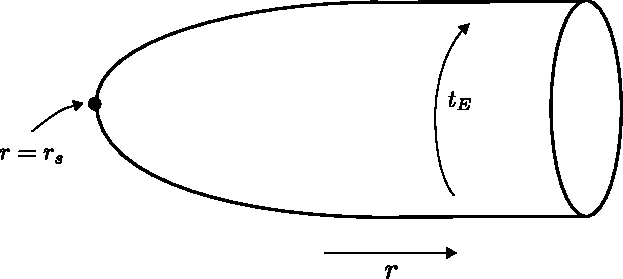
\includegraphics[scale=1]{figures/cigar.pdf}
\end{center}
\caption{\small  The Euclidean Schwarzschild black hole. The Euclidean time and radial directions have the geometry of a cigar, which is smooth at the tip, $r=r_s$. At each point we also have a sphere of radius $r$. \label{fig:cigar}}
\end{figure}

Similarly, in a black hole spacetime, the partition function at inverse temperature $\beta$ is calculated by a Euclidean path integral. The geometry is the Euclidean black hole, obtained from the Schwarzschild metric \eqref{schw} by setting $t = i t_E$,
\be \la{EuclBH}
ds^2_E = \left( 1 - \frac{r_s}{r} \right) dt_E^2 + \frac{dr^2}{1 - \frac{r_s}{r}} + r^2 d\Omega_2^2 \ , ~~~~~~~~~~ t_E = t_E + \beta \ .
\ee
In the Euclidean geometry, the radial coordinate is restricted to $r> r_s$, because we saw that $r-r_s$ is like the radial coordinate in polar coordinates, and $r=r_s$ is the origin   $-$ Euclidean black holes do not have an interior. In order to avoid a conical singularity at $r=r_s$ we need to adjust $\beta$ to 
\be 
\beta = 4 \pi r_s  \ .
\ee
 This geometry, sometimes called the `cigar,' is pictured in fig.~\ref{fig:cigar}. The tip of the cigar is the horizon. Far away, for $r \gg r_s$, there is a Euclidean time circle of circumference $\beta$, which is the inverse temperature as seen by an observer far away. Notice that in the gravitational problem we fix the length of the circle far away, but we let the equations determine the right radius in the rest of the geometry. 

The Euclidean path integral on this geometry is interpreted as the partition function,
\be
Z(\beta)  = \mbox{Path integral on the Euclidean black hole} \sim  e^{ - I_{\rm classical}} Z_{\rm quantum}  \ .
\ee
It has contributions from both gravity and quantum fields. The gravitational part comes from the Einstein action, $I$,  and is found by evaluating the action on the geometry \nref{EuclBH}. The quantum part is obtained by computing the partition function of the quantum fields on this geometry \nref{EuclBH}.
It is important that the geometry is completely smooth at $r=r_s$ and therefore the quantum contribution has no singularity there. 
 This is related to the fact that an observer falling into an evaporating  black hole sees nothing special at the horizon, as in the classical theory. 
 
 Then applying the standard thermodynamic formula to the result,
\be
S = (1 - \beta \p_\beta) \log Z(\beta)
\ee
gives the generalized entropy \eqref{sgen}. We will not give the derivation of this result but it uses that we are dealing with a solution of the equations of motion and that the non-trivial part of the variation can be concentrated near 
$r=r_s$  \cite{Gibbons:1977mu }.  

\subsection{Evaporating black holes}


\begin{figure}[p!]
\begin{center}
\begin{overpic}[grid=false,scale=1]{figures/evap-stagesc.pdf}
\put(150,1050){ 
\parbox[t]{4in}{\centering \Large Stages of Black Hole Evaporation}
}
\put(50,950) {
\parbox[t]{2in}{$(a)$  After stellar collapse,
the outside of the black hole is nearly stationary, but on the inside, the geometry continues to elongate in one direction while pinching toward zero size in the angular directions.
}}
\put(50,720) {
\parbox[t]{4in}{
$(b)$
The Hawking process creates entangled pairs, one trapped behind the horizon
and the other escaping to infinity where it is observed as (approximate)
blackbody radiation. 
}}
\put(50,535) {
\parbox[t]{2in}{
The black hole slowly shrinks as its
mass is carried away by the radiation.
}}
\put(50,340) {
\parbox[t]{3.5in}{
$(c)$ Eventually the angular directions shrink to zero size. This is the singularity. The event horizon also shrinks to zero.
}}
\put(50,150) {
\parbox[t]{3.5in}{
$(d)$ At the end there is a smooth spacetime containing thermal Hawking radiation but no black hole.
}}
\end{overpic}
\end{center}
\caption{ \label{fig:evap-stages}}
\end{figure}


\begin{figure}
\begin{center}
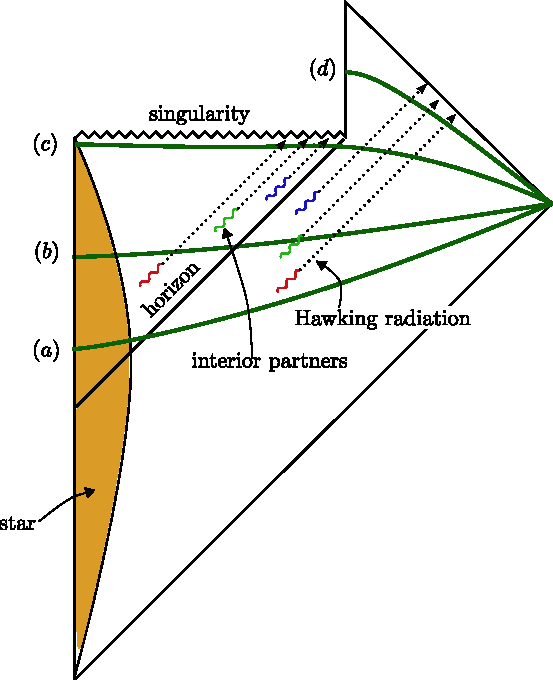
\includegraphics[scale=1]{figures/evap-penrose.pdf}
\end{center}
\caption{Penrose diagram for the formation and evaporation of a black hole. Spatial slices $(a)$-$(d)$ correspond to the slices drawn in fig.~\ref{fig:evap-stages}. \label{fig:evap-penrose}}
\end{figure}


Hawking radiation carries energy away to infinity and therefore reduces the mass of the black hole. Eventually the black hole evaporates away completely --- a primordial black hole of mass $10^{12}\,$kg, produced in the early universe, would evaporate around now. The Hawking temperature of a solar mass black hole is $10^{-7}\,$K and its lifetime is $10^{64}$ years. 
The spacetime for this process is described in figures \ref{fig:evap-stages} and \ref{fig:evap-penrose}.


The Hawking process can be roughly interpreted as pair creation of entangled particles near the horizon, with one particle escaping to infinity and the other falling toward the singularity. This creation of entanglement is crucial to the story and we will discuss it in detail after introducing a few more concepts.


